\chapter{结语与展望}\label{ch:epilogue}

\epigraph{\textit{抽象的目的不是要含糊其辞，而是要创造一个新的语义层次，在其中可以做到绝对精确。}}{Edsger W.\ Dijkstra}

本书的每一章都在讨论同一件事：概率质量在某种预设变换下如何流动，以及如何逆转、近似或利用这种流动来生成数据。在这最后一章中，我们退后一步，把这种结构上的统一性明确地呈现出来。我们首先回顾支撑前述全部内容的变量替换原理（\Cref{sec:epilogue-backbone}），然后说明同样的概率传输视角如何通过马尔可夫核和连续时间马尔可夫链扩展到离散状态空间（\Cref{sec:epilogue-discrete}），最后对更广阔的图景作若干反思（\Cref{sec:epilogue-closing}）。

\clearpage
\newpage

\section{密度传输的主干}\label{sec:epilogue-backbone}

在全书之中，我们沿着两条紧密相关的发展线索展开。
第一条线索是\emph{扩散模型本身}，包括变分、基于分数和基于流这几种形式，它们为概率律如何演化、以及如何为了生成而逆转这种演化提供了不同的数学描述。
第二条线索是\emph{受扩散启发的快速生成器}，其中最具代表性的是流映射模型（flow map models），它们建立于同样的传输视角之上，但旨在学习更直接、更高效的生成器。
尽管形式各异，所有这些方法都根植于同一个组织性思想：生成式建模从本质上讲是一个\emph{传输概率质量}的问题。从一个简单的参考分布（例如高斯噪声）出发，我们设法构造一个过程，逐步把它与复杂的数据分布联系起来。

这种视角之所以有用，是因为它把注意力从单个模型族移开，引向一个更根本的问题：
\emph{当底层样本被某种预设的动力学所驱动时，概率律会如何演化？}
回答这一问题的数学语言，就是变量替换公式及其连续时间推广。从这个意义上说，变量替换原理不仅是一种技术工具，它更是扩散模型及其所启发的快速生成器共同的概念主干。

\paragraph{共同的三步结构。}
在较高的层面上，本书所研究的方法都遵循同样一个简单的模式：
\begin{enumerate}[leftmargin=2em]
    \item 定义一个前向过程，逐步把数据推向一个简单的参考分布。
    \item 通过适当的定律演化方程，理解概率律在该过程下如何演化。
    \item 学习一个生成机制，使之逆转、近似或以其他方式利用这种演化，从而产生样本。
\end{enumerate}
不同形式之间的差别，仅在于前向过程的选择、定律演化方程的数学形式，以及生成机制被参数化和训练的方式。

\paragraph{变量替换的层级体系。}
在 \Cref{app:continuity} 中，我们系统地推导了变量替换公式的一个递进体系，从确定性双射到随机微分方程。这一递进关系值得在此回顾，因为它揭示了同一种传输原理以若干不同形式出现。

\FloatBarrier % ensures figures above don’t float past here

\begin{figure}[H]
  \centering

  % --- First row ---
  \begin{subfigure}{\textwidth}
    \centering
    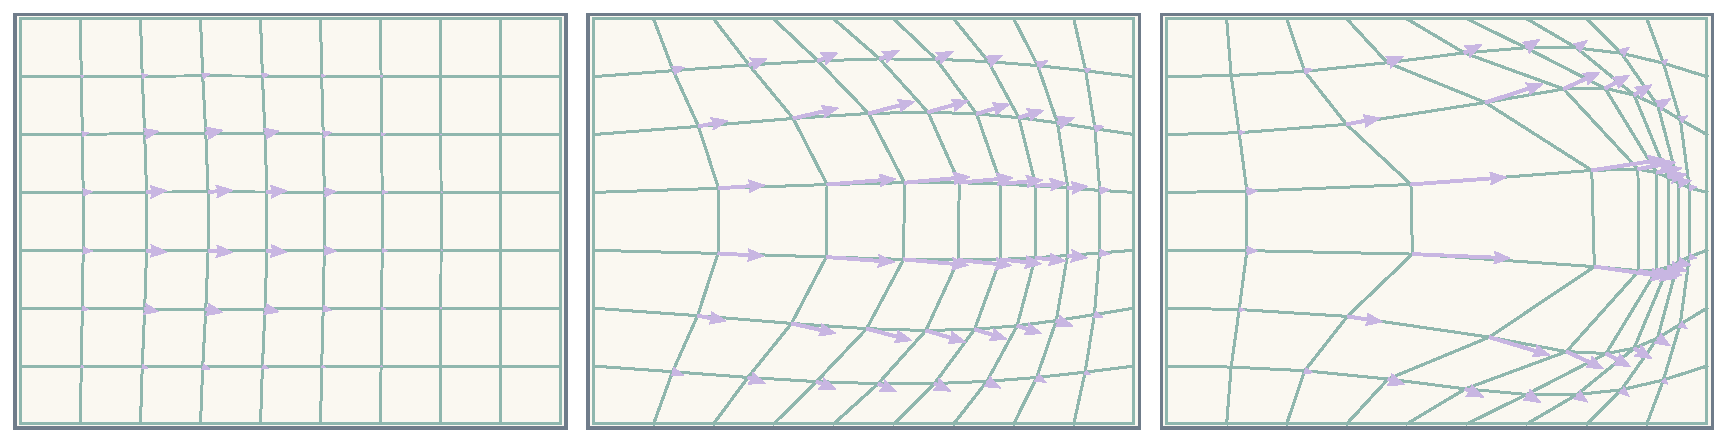
\includegraphics[width=\textwidth]{Images/appendix/vector_field_only.pdf}
        \caption{向量场示意图。箭头代表驱动粒子在空间中运动的力，相应地使底层网格发生形变。}
  \end{subfigure}

  \vspace{0.5em} % space between rows

  % --- Second row ---
  \begin{subfigure}{\textwidth}
    \centering
    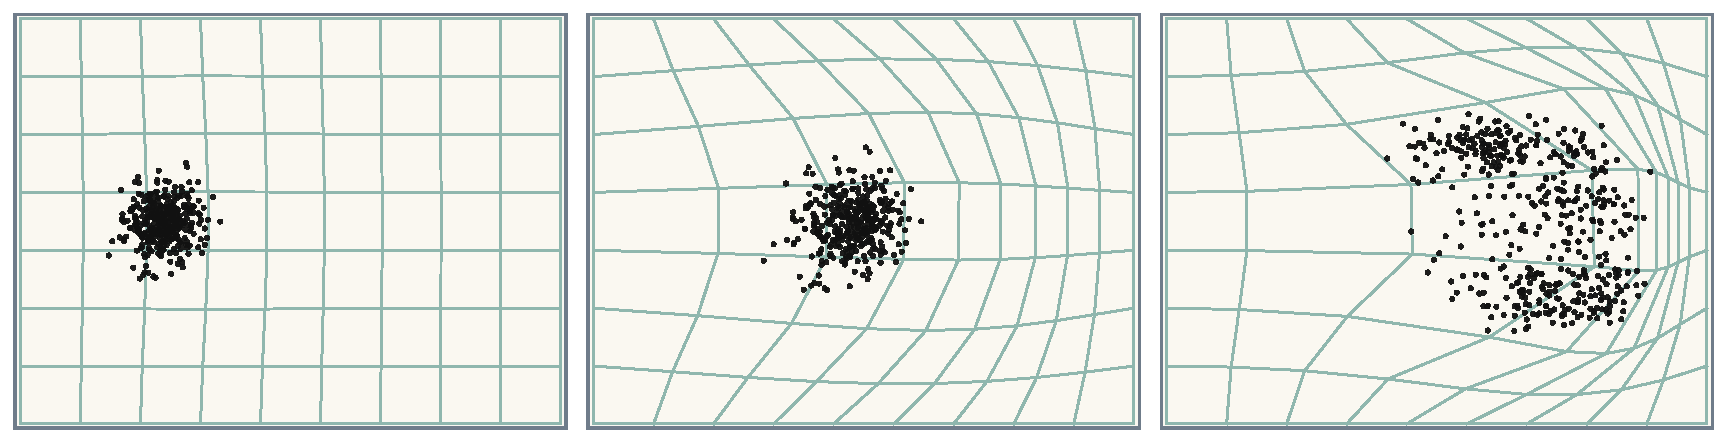
\includegraphics[width=\textwidth]{Images/appendix/particle_cloud.pdf}
    \caption{粒子云动力学。将一个预定义的向量场解释为力，它生成一个流，把粒子从其初始状态传输出去。}
  \end{subfigure}

  \vspace{0.5em}

  % --- Third row ---
  \begin{subfigure}{\textwidth}
    \centering
    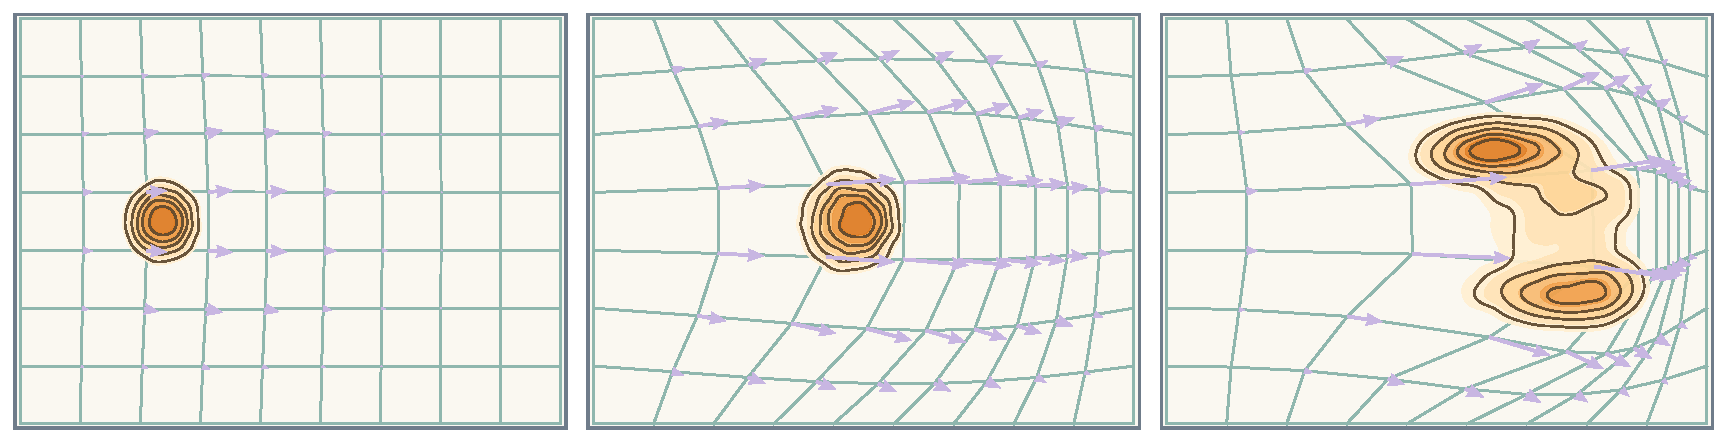
\includegraphics[width=\textwidth]{Images/appendix/vector_field_with_density.pdf}
    \caption{密度演化。当粒子被向量场平流输送时，密度等值线随之形变，反映出流如何重塑底层分布。}
  \end{subfigure}

  \caption{\textbfs{向量场下粒子与密度动力学示意图。}
每一列从左到右依次展示连续的时间快照。\figcredit{改编自 \citet{lipman2024flow}。}
}
  \label{fig:flow-3x3rows}
\end{figure}

\begin{enumerate}[leftmargin=2em]
    \item \textbfs{单个双射。}
    一个光滑可逆映射 $\bPsi:\R^D\to\R^D$ 通过下式把密度 $p_0$ 变换为 $p_1$：
    \[
    p_1(\rvx_1)
    =
    p_0\bigl(\bPsi^{-1}(\rvx_1)\bigr)
    \left|\det \partial_{\rvx_1}\bPsi^{-1}(\rvx_1)\right|.
    \]
    Jacobi 行列式记录了局部的体积变化：当映射拉伸空间时，密度减小；当它压缩空间时，密度增大。

    \item \textbfs{复合双射。}
    把许多双射链接起来，令 $\rvx_k=\bPsi_k(\rvx_{k-1})$，得到
    \[
    \log p_L(\rvx_L)
    =
    \log p_0(\rvx_0)
    -
    \sum_{k=1}^L
    \log\left|\det \partial_{\rvx_{k-1}}\bPsi_k(\rvx_{k-1})\right|.
    \]
    这是归一化流背后的基本原理。更重要的是，它已经阐明了核心信息：一旦粒子运动被确定，密度的演化便随之确定。

    \item \textbfs{连续时间确定性流（ODE）。}
    取无穷小步长的极限，便得到连续性方程，
    \[
    \frac{\partial p_t(\rvx)}{\partial t}
    +
    \nabla\cdot\bigl(p_t(\rvx)\,\rvv(\rvx,t)\bigr)
    =
    0,
    \]
    其中粒子按如下方式演化
    \[
    \frac{\diff \rvx(t)}{\diff t} = \rvv(\rvx(t),t).
    \]
    这是质量守恒的连续时间表达。概率质量既不会被创造也不会被消灭，它只是在速度场 $\rvv$ 之下在空间中流动。

    \item \textbfs{连续时间随机流（SDE）。}
    加入布朗噪声，便得到 Fokker--Planck 方程，
    \[
    \frac{\partial p_t(\rvx)}{\partial t}
    =
    -\nabla\cdot\bigl(\rvv(\rvx,t)\,p_t(\rvx)\bigr)
    +
    \frac{1}{2}g^2(t)\,\Delta p_t(\rvx),
    \]
    它对应于如下的随机动力学
    \[
    \diff\rvx(t) = \rvv(\rvx(t),t)\diff t + g(t)\diff\rvw(t).
    \]
    第一项描述由漂移项驱动的定向传输，第二项刻画噪声引起的随机扩散。
\end{enumerate}

这些并不是互不相关的公式。
多层变量替换法则是重复的确定性变换下传输的离散时间版本。
其无穷小的确定性极限给出连续性方程。
加入随机扰动则导出 Fokker--Planck 方程。
每一层都是对前一层的推广，同时保留了同一个底层原理：概率质量守恒，概率律据此调整，以反映底层动力学如何驱动样本在空间中运动。

从这一视角出发，本书中的主要形式便更容易在整体中定位。
变分方法通过时间网格上的去噪转移来描述生成。基于分数的方法则处理随机动力学，并学习控制逆向时间 SDE 的分数场。
基于流的方法处理确定性传输，并学习一个速度场，其轨迹遵循同一族中间定律。
而快速生成器则建立在这同一主干之上，但寻求更直接的方式来利用所学到的传输以进行高效采样。

因此，核心结论十分简单。
扩散建模最好不应被理解为某个绑定于单一架构或单一噪声调度的单一算法。它是一种\emph{设计原理}：指定一个前向传输过程，理解由此引起的概率律演化，然后在这一结构之上构造一个生成器。一旦确立了这种视角，许多看似不同的方法便成为同一思想的不同自然变体。

随之产生一个自然的问题：这一原理是否可以推广到连续状态空间之外？在下一节中，我们将说明确实如此。

\clearpage
\newpage


\section{超越连续状态：离散空间上的概率演化}
\label{sec:epilogue-discrete}

到目前为止，本书中出现的每一个模型都共享一个共同的结构
假设：生成动力学所作用的状态处于
连续的欧几里得空间 $\R^D$ 之中。不论 $\rvx$ 的各分量代表
像素强度、音频采样还是连续的隐变量，其
数学都是相同的：粒子沿着由 ODE 或 SDE 所支配的连续轨迹运动，而概率密度则通过连续性或
Fokker--Planck 方程演化。这一框架建立在 $\R^D$ 的微分结构之上：梯度与
散度通过导数来定义，确定性动力学可由向量场生成的可微轨迹来描述。

这种区别关乎的是建模所用的状态，而非原始的模态。
离散的观测也可以通过先选择一个连续的编码
和一个读出来处理。对于一个原始符号 $a$，令 $\rmE(a)\in\R^d$ 为其编码，
并令 $\rmD$ 把编码映射回符号，或者更一般地映射到一个
类别分布：
\[
\text{raw discrete symbol } a
\;\xrightarrow{\;\rmE\;}\;
\text{continuous code } \rmE(a)\in\R^d
\;\xrightarrow{\;\rmD\;}\;
\text{discrete readout}.
\]
该表示可以是固定的，例如 one-hot、类别向量或
单纯形取值的编码~\citep{richemond2022categorical}；
在单射码本上，读出可以是确定性的，并可能满足
$\rmD(\rmE(a))=a$。另一种选择是，该表示也可以是学习得到的，
例如词元嵌入或自编码器的隐表示
\citep{li2022diffusionlm,dieleman2022continuous}；此时 $\rmD$ 是一个学习得到的
读出，$\rmD\circ\rmE$ 也不必精确可逆。一旦
表示被固定下来，扩散过程便是连续状态的：在周围编码空间中的高斯加噪，或在受限编码空间中采用几何适配的连续过程，都可以用本书前文所发展的连续机制来处理。下文研究的有限状态路径则不同：演化的状态本身始终保持离散。

本节研究的是与之互补的情形，即在整个前向和反向过程中，状态本身
始终是有限且离散的。许多数据类型天然符合这一视角：文本是词表词元的序列，分子图使用有限多种原子类型和键类型，
蛋白质序列是有限字母表上的字符串。在这样的有限状态
空间中，从一个状态到另一个状态之间不存在规范的无穷小位移，
不存在穿越词元取值的光滑轨迹，也不存在关于状态本身的普通梯度。这自然引出一个问题：
\begin{question}
    如果扩散确实是关于传输概率质量的，那么当状态空间有限时，这一想法会变成什么？
\end{question}

结构主干保持不变，但数学对象发生了变化。
在连续空间中，概率律通过 ODE/SDE 动力学在连续性或
Fokker--Planck 方程下演化。在有限状态空间中，概率质量
按照马尔可夫转移核或跳变速率在状态之间转移，
而定律则由一个有限维的守恒律——即\emph{主方程}，也称为 Kolmogorov 前向方程——所演化。在抽象层面上，
两种设定都遵循同样的配方：

\msg{观察}{}{选择一个前向破坏过程，理解其诱导的概率路径，并学习一个反向传输机制。}

在连续高斯扩散中，这种反向机制表现为高斯
反向条件分布、分数或速度场。在有限状态空间中，它
则表现为反向转移概率、概率比率或跳变
速率。它们是不同的数学对象，但扮演着相同的概念角色。

本章的目标并不在于把某一种离散扩散算法奉为定论。
相反，我们要发展出一份即使文献更迭也应当保持稳定的路线图。该路线图按照用来描述反向传输的对象来组织：转移核、概率比率或跳变速率。我们分四步展开：离散时间转移（\Cref{subsec:epilogue-dtmc}）、其连续时间极限（\Cref{subsec:epilogue-ctmc}）、与连续情形下变分、分数/比率和流三种视角相对应的三种反向建模视角（\Cref{subsec:epilogue-three-views}），以及对离散与连续情形之间真正差异的比较（\Cref{subsec:epilogue-genuine-diff}）。

\subsection{离散时间转移}
\label{subsec:epilogue-dtmc}

考虑一个在 $K$ 个离散类别上的前向过程，其中 $K$
包括所选前向过程所需的任何特殊破坏词元，例如掩码词元。每个状态表示为一个
\emph{one-hot} 列向量 $\rvx\in\{0,1\}^{K}$，其中恰好有一个
分量等于~$1$；所有这种向量的集合为\footnote{在 CTMC 与随机过程文献~\citep{norris1998markov,kelly1979reversibility} 中的一种等价表述，把每个状态表示为一个标量索引 $x\in\{1,\dots,K\}$，把转移
速率写作 $[\rmQ_t]_{ij}$，把边缘分布写作 $p_t(x)$。这里所采用的 one-hot 编码在记号上等价，但更贴近离散扩散文献~\citep{austin2021structured,sahoo2024simple,lou2024discrete}，其中诸如 $\langle\rvx_{\bphi},\rvx\rangle$ 的内积和
诸如 $\rmP^{\top}\rvx$ 的矩阵--向量乘积会自然出现在
训练目标中。}
\[
\mathcal{V}
= \bigl\{\rvx\in\{0,1\}^{K}:\textstyle\sum_{i=1}^{K}x_i=1\bigr\}
= \{\rve_1,\ldots,\rve_K\}.
\]
我们把 $\rve_i$ 记作第 $i$ 个标准基向量，即类别~$i$ 的 one-hot
编码。例如，每个 $\rve_i$ 可以代表
一个词元、一个离散隐码、一种原子类型、一种键类型或一种氨基酸。

对于文本或蛋白质等序列数据，一个样本由 $N$
个词元组成，每个词元在大小为~$K$ 的词表中取值。完整的状态空间便是 $\mathcal{V}^N$，其规模随序列长度呈指数增长。在许多离散扩散模型中，\emph{前向}破坏在各个位置上独立作用，因此单词元的马尔可夫过程便是基本的局部构件。我们先聚焦于单个词元，因为这能揭示核心的概率传输机制而不带来记号上的负担。对于完整序列，同样的公式可应用于完整构型，或者在前向破坏可分解时按位置分解。然而，学习得到的反向模型不必在各位置间独立：Transformer 或图神经网络可以观察整个被破坏的对象，并利用全局上下文来预测局部或全局的反向转移。

\begin{figure}[th!]
    \centering
    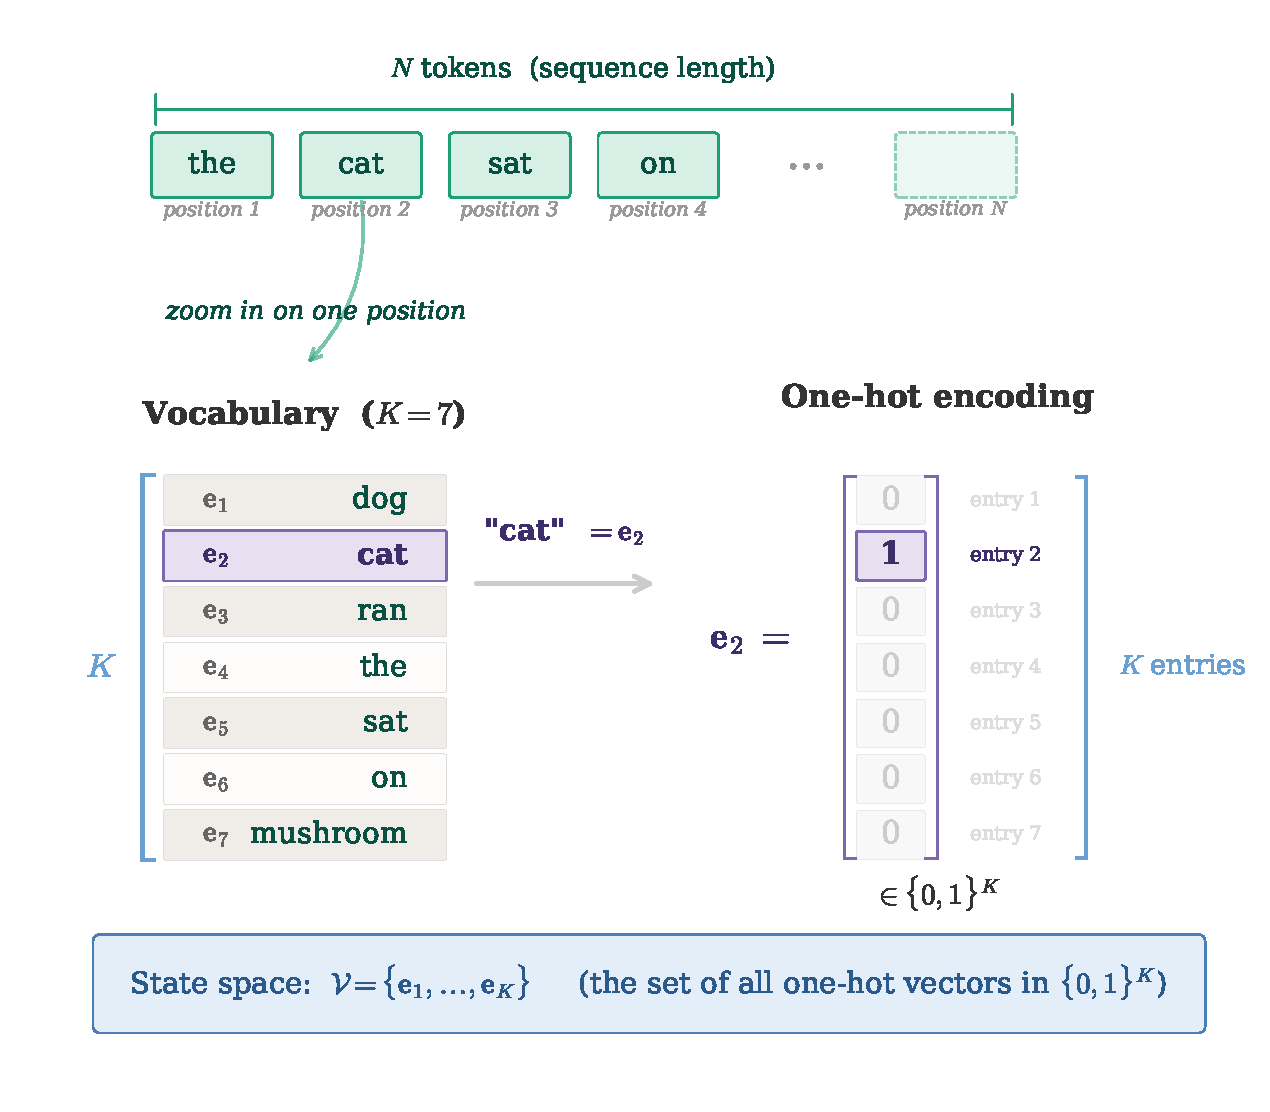
\includegraphics[width=\linewidth]{Images/PartE/fig_notation_overview.pdf}
    \caption{\textbfs{从序列到 one-hot 状态。}
    诸如文本或蛋白质序列这样的数据样本由 $N$
    个词元构成，每个词元在大小为~$K$ 的有限字母表或词表中取值。本章聚焦于
    单个词元在 $K$ 个状态之间的演化。放大观察某个位置，
    这里是 ``cat''，该词元由基向量
    $\rve_2$ 表示，并被编码为 $\{0,1\}^K$ 中的一个 one-hot 向量，即一个
    $K$ 维向量，其第二个分量为~$1$，其余所有
    分量均为~$0$。状态空间
    $\mathcal{V}=\{\rvx\in\{0,1\}^K:\sum_{i=1}^K x_i=1\}
    =\{\rve_1,\ldots,\rve_K\}$ 是所有这种 one-hot 向量的集合。
    词表条目的排序是任意的，与词元在序列中的位置无关。\figcredit{由作者在 AI 辅助编程下绘制。}}
    \label{fig:notation-overview}
\end{figure}

在第~$k$ 步，系统占据这 $K$ 个状态之一。我们把处于
状态~$\rve_i$ 的标量概率记为
\[
p_k(i) := \Pr(\rvx_k=\rve_i),
\qquad i=1,\ldots,K.
\]
收集这些标量概率，便得到边缘概率向量
\[
\rvp_k
:=
\bigl(p_k(1),\;\dots,\;p_k(K)\bigr)^\top
=
\E[\rvx_k]
\in \Delta^{K-1}\subset\R^K,
\qquad
\sum_{i=1}^K p_k(i)=1,
\]
其中 $\Delta^{K-1}:=\bigl\{\rvp\in\R^K:p_i\geq0,\;
\sum_{i=1}^K p_i=1\bigr\}$ 表示概率单纯形。
等价地，$\Pr(\rvx_k=\rve_i)=p_k(i)$，或简记为
$\rvx_k\sim\mathrm{Cat}(\rvp_k)$。

因此 $\rvp_k$ 是离散随机状态 $\rvx_k$ 的完整定律，而
$p_k(i)$ 是其第 $i$ 个标量分量。在连续时间下，我们沿用同一约定：
\[
p_t(i):=\Pr(\rvx_t=\rve_i),
\qquad
\rvp_t:=\bigl(p_t(1),\ldots,p_t(K)\bigr)^\top.
\]
向量 $\rvp_t$ 是密度的离散类比：它告诉我们总概率
质量如何在 $K$ 个状态之间分布。

按照全书使用的约定，粗体小写字母
（$\rvp$、$\rvx$）表示向量，粗体大写字母（$\rmP$、$\rmQ$）
表示矩阵，而不加粗的带下标量，如 $p_k(i)$、
$[\rmP_k]_{ij}$ 和 $[\rmQ_t]_{ij}$，表示标量分量。不加粗的
$p$ 以随机变量为自变量，如
$p(\rvx_{k-1}|\rvx_k)$，表示在固定前向过程下的概率质量函数或转移
核；$p_{\bphi}$ 表示学习得到的反向模型。



系统如何在状态之间转移？单步转移由一个
\emph{转移矩阵} $\rmP_k \in \R^{K \times K}$ 给出。
其元素 $[\rmP_k]_{ij}$ 给出当前处于
状态~$\rve_i$ 的系统在一步之内转移到状态~$\rve_j$ 的概率：
\[
[\rmP_k]_{ij} \;=\; \Pr(\rvx_{k+1} = \rve_j | \rvx_k = \rve_i).
\]
因此完整的矩阵具有如下结构：
\[
\rmP_k \;=\;
\underbrace{
\begin{pmatrix}
[\rmP_k]_{11} & [\rmP_k]_{12} & \cdots & [\rmP_k]_{1K} \\
[\rmP_k]_{21} & [\rmP_k]_{22} & \cdots & [\rmP_k]_{2K} \\
\vdots & \vdots & \ddots & \vdots \\
[\rmP_k]_{K1} & [\rmP_k]_{K2} & \cdots & [\rmP_k]_{KK}
\end{pmatrix}
}_{\substack{\text{columns: next state } j}}
\quad
\left.
\vphantom{
\begin{pmatrix}
a \\ a \\ \vdots \\ a
\end{pmatrix}
}
\right\}
\text{\footnotesize rows: current state } i.
\]
横向读取第 $i$ 行便回答了这样的问题：``已知系统当前
处于状态 $\rve_i$，落入每个可能的下一状态的概率是多少？'' 因此每一行都是关于目的地的一个概率分布：
\[
[\rmP_k]_{ij} \geq 0
\quad \text{for all } i,j,
\qquad\qquad
\sum_{j=1}^{K} [\rmP_k]_{ij} = 1
\quad \text{for each } i.
\]
非负性条件表明每个转移概率都是合法的，
而行和约束则表明所有离开状态~$\rve_i$ 的质量都被计入：
系统总会到达某个地方。

\paragraph{分布如何演化。}
有了转移矩阵，现在我们提出一个基本问题：如果
系统从分布 $\rvp_k$ 出发，一步之后的分布是什么？答案来自简单的概率核算。
转移之后处于状态~$\rve_j$ 的概率，是
从所有可能的源状态到达~$\rve_j$ 的总质量：
\begin{equation}
p_{k+1}(j) = \sum_{i=1}^K p_k(i)\,[\rmP_k]_{ij}.
\label{eq:discrete-transport-one-step}
\end{equation}
求和中的每一项代表最初位于状态~$\rve_i$ 的
质量，并以从~$\rve_i$ 跳到~$\rve_j$ 的概率作为权重。
写成向量形式，即为
\[
\rvp_{k+1} = \rmP_k^\top \rvp_k.
\]
等价地，给定当前 one-hot 状态~$\rvx_k$ 时下一状态的条件分布为
\[
\Pr(\rvx_{k+1} | \rvx_k)
= \mathrm{Cat}(\rvx_{k+1};\,\rmP_k^\top\,\rvx_k),
\]
因为 $\rmP_k^\top\,\rve_i$ 抽取出 $\rmP_k$ 的第 $i$ 行，其中
包含从状态~$\rve_i$ 出发的转移概率。

按此规则演化的系统被称为\emph{离散时间马尔可夫链}：下一步的分布只依赖于当前分布和转移矩阵，而不依赖于系统是如何到达此处的。它在有限状态下扮演着连续空间中定律演化公式的角色。在那里，一个双射 $\bPsi$ 重塑一个密度，而 Jacobi 行列式对局部体积变化做出补偿。在有限状态空间中，没有需要追踪的体积元素。相反，转移矩阵 $\rmP_k$ 直接规定了有多少概率质量离开每个源状态、到达每个目的地。行和约束保证总概率守恒，正如连续性方程中的散度结构所做的那样。

将其在多步上重复，使用转移矩阵
$\rmP_0, \dots, \rmP_{L-1}$，得到
\begin{equation*}
\rvp_L = \rmP_{L-1}^\top \cdots \rmP_1^\top \rmP_0^\top\, \rvp_0.
\end{equation*}
这对应于
\Cref{eq:cov-multi-layer-nolog} 中的多层变量替换公式。在连续确定性设定中，密度
演化通过 Jacobi 行列式累积；而在这里，
概率向量通过接连的马尔可夫算子传播。
底层的思想是一致的：概率质量通过一串
预设的变换被追踪。

\paragraph{逆转单步。}
给定前向机制，一个自然的问题是如何逆转单步
转移以用于生成。假设系统在第~$k{+}1$ 步被观测到处于状态~$\rve_j$。它在上一第~$k$ 步处于
状态~$\rve_i$ 的概率是多少？这是 Bayes 公式的直接应用：
\begin{align}
\Pr(\rvx_k = \rve_i | \rvx_{k+1} = \rve_j)
= \frac{\Pr(\rvx_{k+1} = \rve_j | \rvx_k = \rve_i)\;\Pr(\rvx_k = \rve_i)}
        {\Pr(\rvx_{k+1} = \rve_j)}  
= [\rmP_k]_{ij}\frac{p_k(i)}{p_{k+1}(j)},
\label{eq:discrete-reverse-kernel}
\end{align}
只要 $p_{k+1}(j)>0$。这是与前向转移~$\rmP_k$ 以及当前边缘定律相关联的离散时间反向核。其形式很直观：在质量本可以到达
状态~$\rve_j$ 的所有途径中，每个源~$\rve_i$ 的贡献与那里原本有多少质量（通过 $p_k(i)$）、以及该跳变有多可能发生（通过 $[\rmP_k]_{ij}$）成正比。\Cref{eq:discrete-reverse-kernel} 中的分子和分母各有清晰的解释：
\begin{itemize}[leftmargin=2em]
    \item \textbfs{分子：}
    项 $[\rmP_k]_{ij}\,p_k(i)$ 是第~$k$ 步处于状态~$\rve_i$、然后在第~$k{+}1$ 步跳到~$\rve_j$ 的联合概率。

    \item \textbfs{分母：}
    项
    \[
    p_{k+1}(j) = \sum_{i'} p_k(i')\,[\rmP_k]_{i'j}
    \]
    是从任何源状态到达状态~$\rve_j$ 的总概率。它充当归一化常数，保证反向概率关于~$i$ 求和为一。
\end{itemize}

关键的一点是，反向核\emph{不是} $\rmP_k$ 的矩阵逆。一个马尔可夫转移可能会把来自多个状态的概率质量合并到一个状态，作为线性映射它不一定是可逆的。概率意义上的反向其实是一个 Bayes 意义上的反向，它不仅依赖于前向转移矩阵，还依赖于边缘分布 $\rvp_k$。这恰好就是生成式建模所面临的困难：$\rvp_k$ 是通过把未知的数据分布推过前向过程而获得的，因此通常没有闭式表达。下文所讨论的反向建模视角，可以理解为表示或学习实现这一 Bayes 反向所需缺失信息的不同方式。

\subsection{连续时间极限：主方程}
\label{subsec:epilogue-ctmc}

在连续空间的故事中，把复合双射的步长缩小到零便得到连续性方程
（\Cref{subsec:cov-continuity-eq}）。同样的极限思想在这里也适用。当
时间步长变得无穷小时，离散时间马尔可夫链便成为连续时间马尔可夫链（CTMC），而分布则按主方程演化。

\begin{figure}[th!]
    \centering
    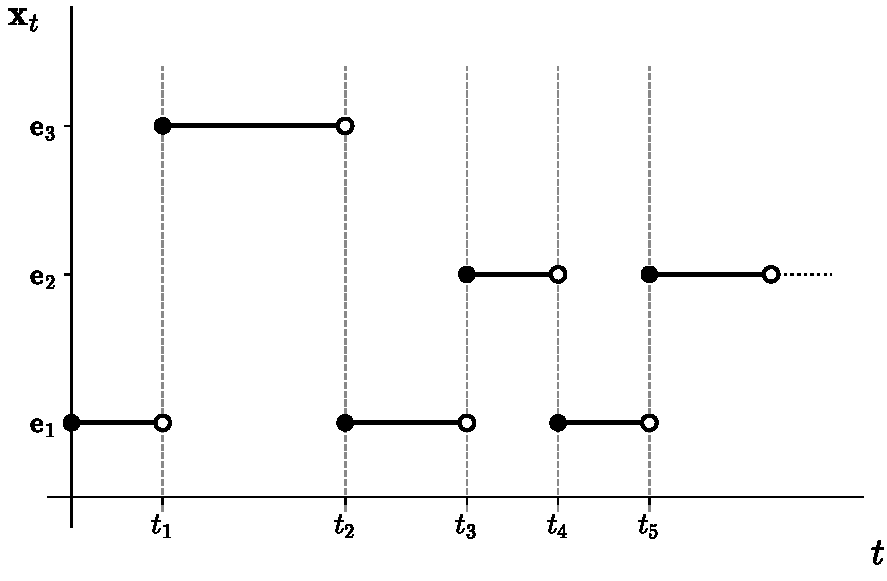
\includegraphics[width=0.8\linewidth]{Images/PartE/ctmc_trajectory.pdf}
    \caption{\textbfs{CTMC 样本路径示意图。}
设状态空间为 $\mathcal{V}=\{\rve_1,\rve_2,\rve_3\}$，在纵轴上标记为 $S_1,S_2,S_3$。
轨迹是分段常值的：过程在 $\rvx_t=\rve_i$ 处停留一段随机的驻留时间，然后在 $t_1,t_2,\ldots$ 等时刻瞬时跳到另一个状态 $\rve_j$。
实心圆圈标记每次跳变后立即占据的状态，空心圆圈标记跳变之前的状态，反映了右连续约定。
虚线段表示超出所显示窗口的延续。
这些跳变时刻和目的地由速率矩阵 $\rmQ_t$ 支配：从状态 $\rve_i$ 出发，过程以瞬时速率 $[\rmQ_t]_{ij}$ 跳到 $\rve_j$（$j\neq i$）。
\figcredit{改编自 \citet{campbell2022continuous}。}}
    \label{fig:ctmc-trajectory}
\end{figure}

\paragraph{无穷小转移。}
在上一小节中，每个转移矩阵 $\rmP_k$ 描述了从时间 $k$ 到时间 $k{+}1$ 的完整一步。现在设想把这些步变得越来越细。令 $\rmP_{t,\Delta t}$ 表示从时间 $t$ 起把系统向前推进一小段时长 $\Delta t$ 的转移矩阵：其元素 $[\rmP_{t,\Delta t}]_{ij}$ 是在区间 $[t,\,t{+}\Delta t]$ 内从状态~$\rve_i$ 转移到状态~$\rve_j$ 的概率。

当 $\Delta t$ 很小时，大部分质量留在原地，只有一小部分发生跳变。这意味着 $\rmP_{t,\Delta t}$ 接近于单位矩阵，可以把它展开为
\begin{equation}
\rmP_{t,\Delta t}
\;=\; \rmI + \rmQ_t\,\Delta t + \mathcal{O}(\Delta t^2),
\label{eq:generator-expansion}
\end{equation}
其中 $\rmQ_t \in \R^{K \times K}$ 是时刻 $t$ 的\emph{速率矩阵}，也称为生成元。如果 $\rmQ_t$ 在时间上足够正则，余项在局部可以写成 $\mathcal{O}(\Delta t^2)$。$\rmQ_t$ 的元素是瞬时
\emph{速率}而非概率。具体而言：
\begin{itemize}[leftmargin=2em]
    \item $[\rmQ_t]_{ij} \geq 0$（$i \neq j$）：这是过程从状态~$\rve_i$ 跳到状态~$\rve_j$ 的速率。乘以 $\Delta t$ 便给出短区间内主导阶的跳变概率。
    \item $[\rmQ_t]_{ii} = -\sum_{j \neq i} [\rmQ_t]_{ij}$：对角元素为负，记录了概率\emph{离开}状态~$\rve_i$ 的总速率。这保证 $\rmQ_t$ 的每一行求和为零，这正是概率守恒在速率层面上的表达。\footnote{这直接来自 $\rmP_{t,\Delta t}$ 的行和约束。由于转移矩阵每一行求和为 $1$，代入展开 $\rmP_{t,\Delta t} = \rmI + \rmQ_t\,\Delta t + o(\Delta t)$ 得到 $1 + \Delta t \sum_{j} [\rmQ_t]_{ij} + o(\Delta t) = 1$，从而迫使 $\sum_{j} [\rmQ_t]_{ij} = 0$。分离出对角项便得 $[\rmQ_t]_{ii} = -\sum_{j \neq i} [\rmQ_t]_{ij}$。}
\end{itemize}
从展开式中读出，在一段短区间内从~$\rve_i$ 跳到 $\rve_j$（$j\neq i$）的概率约为 $[\rmQ_t]_{ij}\,\Delta t$，而留在~$\rve_i$ 的概率约为 $1 - \sum_{j \neq i} [\rmQ_t]_{ij}\,\Delta t$。

\paragraph{主方程。}
有了无穷小转移，连续时间极限便立即得到。把 \Cref{eq:generator-expansion} 中的展开式代入 $\rvp_{t+\Delta t} = \rmP_{t,\Delta t}^\top\,\rvp_t$，并令 $\Delta t \to 0$，得到
\begin{mdframed}
\begin{equation}
\frac{\diff}{\diff t}\,\rvp_t = \rmQ_t^\top\,\rvp_t.
\label{eq:master-equation-vector}
\end{equation}
\end{mdframed}
这是\emph{主方程}，对 CTMC 而言也称为\emph{Kolmogorov 前向方程}~\citep{norris1998markov}。回忆 $\rvp_t$ 是概率向量，其第 $j$ 个分量 $p_t(j)$ 给出在时刻~$t$ 处于状态~$\rve_j$ 的概率。把 \Cref{eq:master-equation-vector} 的第 $j$ 个分量写出来，其含义便很具体：
\begin{equation}
\frac{\diff}{\diff t}\,p_t(j)
= \underbrace{\sum_{i \neq j} p_t(i)\,[\rmQ_t]_{ij}}_{\text{inflow: mass arriving from other states}}
\;-\;
\underbrace{p_t(j)\sum_{\ell \neq j} [\rmQ_t]_{j\ell}}_{\text{outflow: mass departing to other states}}.
\label{eq:master-equation-component}
\end{equation}
$p_t(j)$ 的变化率就是流入减去流出。这就是以微分方程形式表达的概率守恒。

\paragraph{与连续性方程的比较。}
在连续空间中，连续性方程
\[
\partial_t\,p_t(\rvx) + \nabla \cdot
\big(p_t(\rvx)\,\rvv(\rvx,t)\big) = 0
\]
表明密度的变化由速度场 $\rvv$ 之下的概率质量净通量所驱动。主方程用有限状态的语言讲述了同样的事情：$p_t(j)$ 由于速率矩阵 $\rmQ_t$ 所支配的概率净通量而变化。速度场和速率矩阵扮演着类似的结构角色：二者都规定了概率质量如何被重新分配，并且都强制守恒。主要区别是几何上的：在 $\R^D$ 中，质量通过相邻的空间位置流动；在有限状态空间中，质量沿着转移图的允许边跳变。

\begin{figure}[th!]
    \centering
    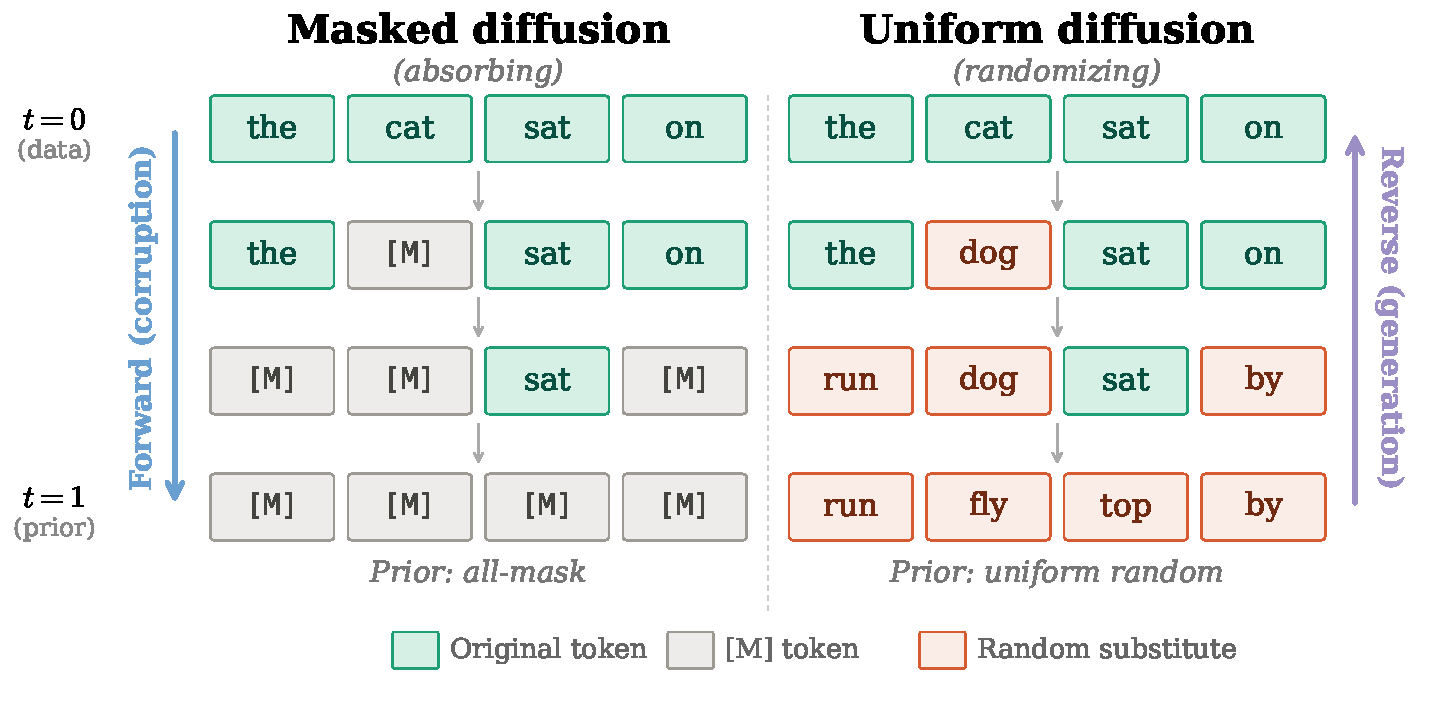
\includegraphics[width=\linewidth]{Images/PartE/masked_vs_uniform_diffusion.pdf}
\caption{\textbfs{掩码扩散与均匀扩散的前向破坏和反向生成示意图。}
这里所示的两个例子都允许形如
$\Pr(\rvx_t|\rvx_0)=\mathrm{Cat}(\rvx_t;\alpha_t\rvx_0+(1-\alpha_t)\bm{\pi})$
的插值边缘分布，其中极限先验 $\bm{\pi}$ 和衰减因子 $\alpha_t$ 由所选的前向速率矩阵决定。在掩码扩散中，词元被吸收到掩码状态，极限先验为 $\bm{\pi}=\rvm=\rve_K$。在均匀扩散中，词元被反复随机化，极限先验为 $\bm{\pi}_{\mathrm{unif}}=\frac{1}{K}\mathbf{1}$。生成过程逆转所选的破坏过程，从对应的简单参考分布出发，或从其有限的有限时间近似出发。
\figcredit{由作者在 AI 辅助编程下绘制。}}
    \label{fig:mask-uniform}
\end{figure}

\paragraph{前向破坏。}
正如连续情形那样，我们需要一个前向过程，逐步破坏数据分布的结构，并将其推向一个易于采样的简单参考分布。这是连续扩散中选择高斯加噪过程的离散类比。设计目标是一致的：破坏应当是渐进的、在解析上或计算上易于处理的，并且足够强，以至于到终止时刻 $T$ 时，数据分布已被基本冲刷掉。

速率矩阵可以有许多选取方式。它可以是均匀的、吸收的、最近邻的、基于图的、化学结构的、语法感知的，或者是为数据领域作其他适配的。下面的两个例子因此并非旨在穷尽分类；它们是让机制变得透明可见的典型情形。
\subparagraph{掩码扩散（吸收式）。} 把最后一个类别保留为掩码词元，记为 $\rvm := \rve_K$。干净数据 $\rvx_0$ 占据前 $K{-}1$ 个类别之一，故 $\langle\rvx_0,\rvm\rangle = 0$。速率矩阵如此定义：每个普通状态以速率 $\beta(t)$ 转移到掩码状态，而掩码状态从不向外转移：
\[
[\rmQ_t]_{iK}=\beta(t),\qquad
[\rmQ_t]_{ii}=-\beta(t),\qquad
[\rmQ_t]_{ij}=0
\quad
\text{for } i<K,\; j\notin\{i,K\},
\]
和
\[
[\rmQ_t]_{Kj}=0
\quad
\text{for all } j.
\]
其想法很简单：每个词元以速率 $\beta(t)$ 独立地被替换为掩码，一旦被掩码便保持掩码。

以干净状态 $\rvx_0$ 为条件的前向边缘分布为
      \[
      \Pr(\rvx_t | \rvx_0)
      = \mathrm{Cat}\bigl(\rvx_t;\;
          \alpha_t\,\rvx_0 + (1-\alpha_t)\,\rvm\bigr),
      \]
      其中
      \[
      \alpha_t
      =
      \exp\left(-\int_0^t\beta(s)\,\diff s\right).
      \]
在时刻~$t$，词元以概率 $\alpha_t$ 等于其干净值 $\rvx_0$，以概率 $1-\alpha_t$ 被掩码。随着时间增长，越来越多的概率质量聚集在掩码状态上。如果 $\int_0^T\beta(s)\diff s$ 很大，那么 $\alpha_T$ 很小，终止分布便接近全掩码的参考分布。

\subparagraph{均匀扩散。} 这一过程不是擦除一个词元，而是逐步将其随机化。一种方便的连续时间归一化方式是让一个词元以相同速率跳到其他 $K-1$ 个状态中的每一个：
      \[
      [\rmQ_t]_{ij} = \frac{\beta(t)}{K - 1}
      \quad\text{for } i \neq j,
      \qquad
      [\rmQ_t]_{ii} = -\beta(t).
      \]
第一个公式说，从状态 $\rve_i$ 出发，词元以相同的瞬时速率跳到每一个备选状态。第二个公式说，离开状态 $\rve_i$ 的总速率为 $\beta(t)$。

前向边缘分布再次取插值形式
      \[
      \Pr(\rvx_t|\rvx_0)
      = \mathrm{Cat} \bigl(\rvx_t;\;
          \alpha_t\,\rvx_0 + (1-\alpha_t)\,\bm{\pi}_{\mathrm{unif}}
        \bigr),
      \]
      其中
      $\bm{\pi}_{\mathrm{unif}}=\tfrac{1}{K}\mathbf{1}\in\R^K$ 是
      均匀概率向量。在上述速率归一化下，
      衰减因子为
      \[
      \alpha_t
      =
      \exp\left(
      -\frac{K}{K-1}\int_0^t \beta(s)\,\diff s
      \right).
      \]
随着时间流逝，反复的随机化会冲刷掉数据分布的结构，把它推向 $\mathcal{V}$ 上的均匀分布。

更一般地，前向过程不必具有简单的混合形式
\[
\Pr(\rvx_t|\rvx_0)
= \mathrm{Cat}\bigl(\rvx_t;\;\alpha_t\rvx_0+(1-\alpha_t)\bm{\pi}\bigr).
\]
那种形式对于直观很有用，也出现在常见的掩码构造和均匀构造中，但马尔可夫定律演化的视角更加一般：转移矩阵支配离散时间演化，速率矩阵通过主方程支配连续时间演化。结构化的离散扩散模型可以使用尊重编辑距离、图邻接、分子有效性、词表结构或其他领域知识的转移规则。在所有情形中，同样的原理都保持不变：前向马尔可夫过程定义一条概率路径，而生成则学习沿该路径反向运动。

\subsection{关于反向建模的三种视角}
\label{subsec:epilogue-three-views}

一旦前向过程及其定律演化就位，剩下的任务与连续情形一致：学习一个反向过程，其边缘分布沿逆向时间回溯前向演化，把简单的参考样本变为数据。在 B 部分，
我们把连续扩散模型组织为三种视角：
变分（\Cref{ch:variational}）、基于分数（\Cref{ch:score-based,ch:score-sde}）和基于流
（\Cref{ch:flow-based}）。同样的三分视角也延续到离散设定中，但有一个重要的提醒：它们并非互斥的学派或固定的论文类别。它们是三种识别``为了逆转概率路径必须学习哪个未知对象''的方式。

\paragraph{变分视角：学习反向转移核。}
在连续情形中（\Cref{sec:ddpm}），变分视角
把扩散视为一个层次化的隐变量模型。前向
过程定义了一条噪声越来越大的隐变量链，目标是
学习能够一次一步地解除破坏的反向转移。真实的反向核 $\Pr(\rvx_{k-1}|\rvx_k)$ 难以处理，因为它依赖于 $\rvx_k$ 的边缘定律，而后者涉及
未知的数据分布。DDPM 的关键洞察是以
干净样本 $\rvx_0$ 为条件：前向后验
$\Pr(\rvx_{k-1}|\rvx_k, \rvx_0)$ 是闭式的高斯分布，而
定理~\ref{thm:equiv-marginal-kl} 表明，针对该
条件后验进行训练，等价于（在不依赖于所学反向模型的项的意义下）针对难以处理的边缘反向核进行训练。于是 ELBO
分解为一系列 KL 项之和（\Cref{eq:ddpm-diffusion}），每个噪声层级一项，每一项都要求所学模型去匹配一个易于处理的
前向后验。

同一套逻辑适用于离散设定。把从数据分布中抽取 $\rvx_0$、再施加固定前向链所得到的联合定律记为 $p$，把学习得到的反向模型记为 $p_{\bphi}$。考虑一条被破坏的 one-hot 状态链
\[
\rvx_0 \;\xrightarrow{\;\rmP_0\;}\; \rvx_1 \;\xrightarrow{\;\rmP_1\;}\;
\cdots \;\xrightarrow{\;\rmP_{L-1}\;}\; \rvx_L,
\]
其中 $\rvx_0$ 从数据分布中抽取，而 $\rvx_L$ 接近一个简单的参考分布，例如全掩码或均匀分布。转移
现在是类别型的而非高斯的，但变分结构是相同的：
\begin{itemize}[leftmargin=2em]
    \item 真实的反向 $p(\rvx_{k-1}|\rvx_k)$ 难以处理，
      因为它依赖于第~$k$ 步的边缘分布。
    \item 以 $\rvx_0$ 为条件，可通过 Bayes 公式使前向后验变得易于处理：
      \[
      p(\rvx_{k-1}|\rvx_k, \rvx_0)
      =
      \frac{p(\rvx_k|\rvx_{k-1})\;p(\rvx_{k-1}|\rvx_0)}
             {p(\rvx_k|\rvx_0)},
      \]
      其中右侧的每个因子都由前向过程决定。
    \item 针对这些条件后验的训练与针对难以处理的边缘反向核的训练具有相同的最佳反向核；二者的差异仅在于一些与 $p_{\bphi}$ 无关的项。
\end{itemize}

示意性地，离散扩散 ELBO 含有如下形式的去噪项
\[
\E_{p(\rvx_{0:L})}
 \Big[
\mathcal{D}_{\mathrm{KL}} \big(
  p(\rvx_{k-1}|\rvx_k, \rvx_0)
  \;\|\;
  p_{\bphi}(\rvx_{k-1}|\rvx_k)
\big)
\Big],
\qquad k=1,\ldots,L.
\]
根据具体模型的不同，完整的 ELBO 还可能包含边界项，例如终止先验项和 $k=0$ 附近的重构项。关键
在于，每个去噪项都要求所学反向核去匹配一个由前向破坏决定的、易于处理的 Bayes 后验。

这里 $p_{\bphi}(\rvx_{k-1}=\rve_i|\rvx_k=\rve_j)$ 表示由神经网络参数化的反向转移概率：给定系统在第~$k$ 步处于状态~$\rve_j$，它给出在第~$k{-}1$ 步来自状态~$\rve_i$ 的概率。对于每个固定的 $\rve_j$，这些值构成关于上一状态的一个类别分布。

与连续 DDPM 的主要形式差别在于，这些 KL 散度是关于离散状态的有限和，而非闭式的高斯表达式。这反映了高斯分布的一个特殊性质：同一变量下两个高斯密度的乘积正比于另一个高斯。在连续 DDPM 中，
前向后验通过高斯因子的相乘来计算，因此结果本身是高斯的，
而 KL 散度简化为只涉及
均值和协方差的简单代数表达式（\Cref{sec:ddpm}）。在离散设定中，
Bayes 公式给出的是类别分布，每个 KL 项都是关于状态的求和。这个和是精确的且在概念上简单，但对于大词表或完整序列空间，它可能需要结构、分解、子采样或专门的参数化。

关于参数化的一个实践要点也值得注意。ELBO 要求所学反向核 $p_{\bphi}(\rvx_{k-1}|\rvx_k)$ 去匹配一个 Bayes 后验，但它并不强制该核的唯一神经参数化。一种常见的选择是干净状态预测，或称 $x_0$-预测
的参数化。精确的边缘反向核满足恒等式
\[
p(\rvx_{k-1}|\rvx_k)
=
\sum_{a}
p(\rvx_{k-1}|\rvx_k,\rvx_0=\rve_a)\,
p(\rvx_0=\rve_a|\rvx_k),
\]
其中求和遍历合法的干净类别。这只是对未知干净状态做边缘化。由于后验 $p(\rvx_0|\rvx_k)$ 依赖于
数据分布，它没有闭式表达。因此，一个模型可以预测一个干净状态分布 $\widehat p_{\bphi}(\rvx_0|\rvx_k)$，并用它来定义
\[
p_{\bphi}(\rvx_{k-1}|\rvx_k)
:=
\sum_{a}
p(\rvx_{k-1}|\rvx_k,\rvx_0=\rve_a)\,
\widehat p_{\bphi}(\rvx_0=\rve_a|\rvx_k).
\]
如果 $\widehat p_{\bphi}(\rvx_0|\rvx_k)$ 等于真实后验
$p(\rvx_0|\rvx_k)$，这个混合便能恢复精确的反向核。在
实践中，这是把所学反向转移与已知的前向后验联系起来的有用方式。

这种干净状态参数化在多项式/D3PM 式
离散时间扩散模型~\citep{hoogeboom2021argmax,austin2021structured} 中很常见，但它并不是离散扩散的定义。D3PM 本身就指出，可以直接预测反向 logits，而后续模型则使用为前向过程量身定制的其他结构化参数化
\citep{sahoo2024simple}。因此，干净状态预测应被视为变分视角下的一种重要参数化，而非建模反向过程的唯一方式。

\paragraph{分数/比率视角：学习局部概率比较。}
在连续情形中（\Cref{ch:score-based,ch:score-sde}），基于分数的视角从一个简单的问题出发：给定一个被破坏的样本 $\rvx_t \sim p_t$，要逆转扩散，需要关于当前密度的什么局部信息？答案是分数函数
$\nabla_{\rvx}\log p_t(\rvx)$，它出现在逆向时间
SDE 和概率流 ODE\@。因此，用神经网络学习分数便足以完成生成。

在有限状态空间中，没有周围的欧几里得几何，没有普通的无穷小位移概念，也没有关于状态的梯度。一个样本不会
通过取一个小的欧几里得步长来运动，而是通过从一个状态跳到另一个状态来改变。
因此分数 $\nabla_{\rvx}\log p_t(\rvx)$ 没有直接的、字面上的类比。但
反向过程仍必须回答一个类似的问题：\emph{如果
系统当前处于状态~$\rve_j$，那么每个候选源状态~$\rve_i$ 相对于它有多可能？}

\subparagraph{推导反向跳变速率。}
为了识别所需的量，考虑一个具有速率矩阵~$\rmQ_t$ 和边缘 $\rvp_t$ 的前向 CTMC $\{\rvx_t\}_{0\leq t\leq T}$。元素 $[\rmQ_t]_{ij}$ 是从
状态~$\rve_i$ 到状态~$\rve_j$ 的跳变速率。在一段短区间~$\Delta t$ 内，
无穷小前向事件
$\rvx_t=\rve_i$ 且 $\rvx_{t+\Delta t}=\rve_j$（$i\neq j$）的概率约为
\[
p_t(i)\,[\rmQ_t]_{ij}\,\Delta t.
\]

现在定义反向时间过程 $\bar{\rvx}_s := \rvx_{T-s}$（$0\leq s\leq T$）。它在反向时间 $s$ 处的边缘为 $\bar{\rvp}_s=\rvp_{T-s}$。如果反向过程具有速率矩阵 $\bar{\rmQ}_s$，那么从 $\rve_j$ 到 $\rve_i$ 的相应反向跳变必须在逆序的时间顺序下重现相同的无穷小路径概率。取极限 $\Delta t\to 0$，得到非对角的时间反演公式
\begin{mdframed}
\begin{equation}
[\bar{\rmQ}_s]_{ji}
= [\rmQ_{T-s}]_{ij}\;\frac{p_{T-s}(i)}{p_{T-s}(j)},
\qquad i \neq j,
\label{eq:reverse-rate-discrete-reverse-time}
\end{equation}
\end{mdframed}
只要 $p_{T-s}(j)>0$。等价地，若 $t$ 表示相应的前向时间，而 $\widetilde{\rmQ}_t$ 表示按该前向时间索引的反向生成元，则有
\begin{equation}
[\widetilde{\rmQ}_t]_{ji}
= [\rmQ_t]_{ij}\;\frac{p_t(i)}{p_t(j)},
\qquad i \neq j.
\label{eq:reverse-rate-discrete}
\end{equation}
对角元素由行和为零的约束所确定，
\[
[\widetilde{\rmQ}_t]_{jj}
=
-\sum_{i\neq j}[\widetilde{\rmQ}_t]_{ji}.
\]
这是 CTMC 的标准时间反演公式
\citep{kelly1979reversibility,anderson2012continuous}，由 \citet{campbell2022continuous} 应用于离散扩散。该公式仅在具有正边缘概率的状态上有意义。此外，
反向过程只沿着前向过程所允许的转移逆转概率通量：如果 $[\rmQ_t]_{ij}=0$，那么从 $\rve_j$ 到 $\rve_i$ 的相应反向速率也为零。该陈述并非一种平衡的细致平衡假设；它是关于无穷小路径概率的局部时间反演恒等式。

\subparagraph{比率作为分数的离散类比。}
现在审视 \Cref{eq:reverse-rate-discrete}。前向速率
$[\rmQ_t]_{ij}$ 是已知的，因为前向过程由设计固定。
未知的量是比率 $p_t(i)/p_t(j)$，
它在当前边缘下比较状态~$\rve_i$ 相对于
状态~$\rve_j$ 有多可能。用内积记号，
$p_t(i) = \langle\rvp_t,\rve_i\rangle$，所以该比率可以写成
$\langle\rvp_t,\rve_i\rangle / \langle\rvp_t,\rve_j\rangle$。

为什么这是分数的离散类比？在连续空间中，
分数 $\nabla_{\rvx}\log p_t(\rvx)$ 度量的是
在一个无穷小位移之下对数密度的变化。在有限状态空间中，
自然的局部比较则跨越一个从一个状态
到另一个状态的允许跳变。沿着从~$\rve_j$ 到~$\rve_i$ 的跳变，对数概率的变化为
\[
\log p_t(i) - \log p_t(j)
= \log \frac{p_t(i)}{p_t(j)},
\]
这是对数概率的有限差分，扮演着
$\log p_t$ 的方向导数在~$\R^D$ 中所扮演的角色。这种比较自然是\emph{边局部的}：该比率只在由前向跳变结构所连接的状态对上才需要。因此，离散分数并不是 $\mathbb{R}^D$ 上的欧几里得向量场；它是沿着允许转移的一系列局部概率比较。对于完整序列，同样的陈述在把 $i$ 和 $j$ 替换为完整构型（通常是 Hamming 型或基于图的转移结构下的相邻构型）后依然成立。

\subparagraph{网络学习什么。}
在连续基于分数的模型中，训练一个神经网络
$\rvs_{\bm{\phi}}(\rvx, t)$ 来逼近分数
$\nabla_{\rvx}\log p_t(\rvx)$，并把所学分数代入
逆向时间 SDE 来生成样本。离散情形在信息层面上遵循同一逻辑：网络必须提供为通过
\Cref{eq:reverse-rate-discrete} 确定反向跳变速率所需的、随时间变化的比率信息。随后，生成通过使用所学转移概率或速率来模拟逆向时间马尔可夫链或 CTMC 进行。

不同的表述以不同方式表示这一信息。基于比率的模型，如 SEDD~\citep{lou2024discrete}
，使用受分数匹配启发的损失来估计比率 $p_t(i)/p_t(j)$ 或其对数形式。其他连续时间表述
\citep{campbell2022continuous,sun2023scorebased} 则通过诸如匹配条件转移概率的目标来学习等价的反向量。把局部概率比较视为分数的离散类比这一想法
由 \citet{meng2022concrete} 的\emph{具体分数}（concrete score）所形式化。
尽管在参数化上有这些差异，底层原理
是共通的：学习时间反演所需的局部概率比较，构造反向转移或速率，并向后模拟。

\paragraph{流视角：学习一个离散传输场。}
在连续情形中（\Cref{ch:flow-based}），基于流的视角
采取的是另一条路径：与其先学分数再逆转
SDE，不如直接学习一个速度场 $\rvv_t(\rvx)$，其 ODE 流
把参考分布传输到数据分布。其
训练策略是流匹配
（\Cref{sec:flow-matching-framework}）：边缘速度场是难以处理的，但一个\emph{条件}速度场
$\rvv_t(\rvx | \rvx_0)$，以数据样本或端点样本为条件，有闭式表达。边缘目标与条件目标通过下式联系：
\[
\rvv_t(\rvx)
= \E \big[\rvv_t(\rvx | \rvx_0) | \rvx_t = \rvx\big],
\]
这是在给定当前状态下对所有可能条件变量的平均。显式计算这一平均需要知道连续边缘
密度 $p_t(\rvx)$。关键的训练技巧（\Cref{subsec:fm-instantiations}）在于，
在平方误差回归下，条件目标与难以处理的边缘目标具有相同的总体最小化子。因此，训练通过使用来自易于处理的条件路径的样本来避开显式的边缘计算。

离散情形遵循同样的想法，只是用速率矩阵替代速度场。由于离散状态无法
沿词元空间中的连续轨迹运动，速度场的角色由一个速率矩阵（也称为马尔可夫生成元）$\rmQ_t$ 来扮演。回忆元素 $[\rmQ_t]_{ij}$ 规定了从状态~$\rve_i$ 到状态~$\rve_j$ 的跳变速率；单位时间内从~$\rve_i$ 实际送到~$\rve_j$ 的概率质量是通量
\[
J_t(i,j)=p_t(i)\,[\rmQ_t]_{ij}.
\]
在这个意义上，速率矩阵是一个离散的传输场：它决定了概率质量如何随时间被重新分配。

这里有一个重要的微妙之处。一条概率路径 $\{\rvp_t\}_{t\in[0,T]}$ 并不唯一地确定一个速率矩阵。许多不同的生成元都可以在主方程中产生相同的导数 $\diff\rvp_t/\diff t$，正如不同的传输场有时也能在不同的几何约束下实现相同的边缘演化。因此，一个离散流匹配方法不仅指定一条概率路径，还要指定一条沿该路径赋予条件跳变速率或概率流的规则。

正如连续流匹配那样，边缘速率矩阵通常是难以处理的，但条件版本往往可以显式给出。如果
以一个端点（例如干净数据状态和/或参考状态）为条件，就可以规定一条条件概率路径，并沿该路径导出易于处理的条件跳变速率。随后，在适当的恰当损失下训练一个神经网络，从被破坏的样本预测相应的转移或速率信息。边缘生成元通过同样的条件期望原理得到：在给定当前状态下对未知端点分布求该条件传输对象的平均，但该平均是通过对条件目标的监督回归或分类来学习，而非显式计算。

与连续流匹配的对应关系如下：
\begin{itemize}[leftmargin=2em]
    \item 在连续流匹配中，网络学习一个条件
      速度场；边缘速度作为流匹配损失下的最佳预测子而涌现。
    \item 在离散流匹配中，网络学习条件
      转移或跳变速率信息；边缘离散传输场通过类似的条件期望机制而涌现。
\end{itemize}
在两种情形中，训练都通过使用易于处理的条件路径和采样的中间状态，来避开难以处理的边缘定律。

这一视角由 \citet{campbell2024generative} 和
\citet{gat2024discrete} 在离散流模型或离散流匹配的名目下发展。更广义地说，流视角应被理解为关于\emph{学习的是什么对象}的陈述：离散状态空间上的一个传输场，由转移、速率或概率流来表示。

\subsection{何者相似，何者真正不同？}
\label{subsec:epilogue-genuine-diff}

下表总结了连续扩散模型与离散扩散模型之间的对应关系。横向阅读每一行，可以看到同一概念成分在两种不同设定下的实例化：

\begin{table}[!t]
\caption{\textbfs{概率传输的连续视角与离散视角。}
同样的生成式建模成分既出现在连续状态空间中，也出现在有限离散状态空间中，但数学对象发生了变化：密度变成概率向量，ODE/SDE 动力学变成马尔可夫链或 CTMC，而反向建模则通过转移核、分数/比率信息或离散传输场来表达。}
\label{tb:continuous-discrete-diffusion}
\centering
\begingroup
\scriptsize
\setlength{\tabcolsep}{4pt}
\renewcommand{\arraystretch}{1.08}
\begin{tabular}{p{0.15\linewidth} p{0.40\linewidth} p{0.40\linewidth}}
\toprule
\textbfs{状态}
& \textbfs{连续} $(\rvx \in \R^D)$
& \textbfs{离散} $(\rvx \in \mathcal{V} \subset \{0,1\}^K)$ \\
\midrule

\textbfs{定律}
& 密度 $p_t(\rvx)$
& 概率向量 $\rvp_t \in \Delta^{K-1}$ \\
\graymidrule

\textbfs{样本 \newline 动力学}
& ODE 或 SDE 轨迹
& 马尔可夫链或 CTMC 跳变 \\
\graymidrule

\textbfs{定律 \newline 演化}
& 连续性方程或 Fokker--Planck 方程
& 转移矩阵传播或主方程 \\
\graymidrule

\textbfs{传输 \newline 对象}
& 速度场、漂移、扩散或分数场
& 转移核、速率矩阵、比率或概率流 \\
\graymidrule

\textbfs{参考 \newline 定律}
& 简单分布，例如高斯
& 简单分布，例如均匀或全掩码 \\

\midrule
\multicolumn{3}{c}{\textbfs{反向建模的三种视角}} \\
\midrule

\textbfs{变分}
& 带有高斯或连续转移的 ELBO
& 带有类别型转移的 ELBO \\
\graymidrule

\textbfs{分数/比率}
& 学习分数 $\nabla_{\rvx}\log p_t(\rvx)$
& 学习比率或对数比率，例如 $p_t(i)/p_t(j)$ \\
\graymidrule

\textbfs{流}
& 学习速度场 $\rvv_t(\rvx)$
& 学习转移、速率或流场 \\

\bottomrule
\end{tabular}
\endgroup
\end{table}
\noindent
这种对应关系很干净，但离散设定
并不仅仅是把连续理论中的梯度替换为比率。有几个更深层的差异值得强调。

\paragraph{没有字面意义上的逆映射。}
在一个确定性连续归一化流中，反向映射就是前向映射的字面意义上的逆。而在离散马尔可夫过程中，前向核可能会合并来自多个状态的质量，因而不必可逆。因此，反向过程不是通过矩阵求逆得到的。它是一种依赖于当前边缘定律的 Bayes 或时间反演构造。这就是反向转移概率中含有诸如 $p_k(i)/p_{k+1}(j)$ 的因子、反向跳变速率中含有诸如 $p_t(i)/p_t(j)$ 的比率的原因。

\paragraph{几何与样本路径。}
在连续欧几里得空间中，单个样本沿
连续时间轨迹演化：ODE 解是光滑的，而 SDE 样本
路径是连续的，尽管通常处处
不可微。这种微分结构使得速度场、分数函数和散度等对象有意义。相比之下，在有限状态空间中，单条轨迹是
\emph{纯跳变路径}：它在一个状态上停留一段随机的驻留时间，然后突然跳到另一个状态。平滑演化的不是样本路径本身，而是概率向量 $\rvp_t$，它按主方程在概率单纯形上随时间连续演化。因此，离散扩散仍然在概率演化的层面上允许一种统一的描述，但其样本层面的动力学由跳变过程支配，而非由数据空间中的连续 ODE/SDE 路径支配。

\paragraph{前向破坏结构与反向参数化。}
在离散扩散中，前向破坏过程往往是一个实质性的建模选择。在连续高斯扩散中，人们可以调整调度 $\alpha_t$ 和 $\sigma_t$，但前向核通常仍是高斯的，因此主要作用是控制破坏的速率与尺度。相比之下，在离散扩散中，转移规则本身可以改变：可以使用均匀破坏、掩码、最近邻转移、图结构转移、领域专用转移，或更一般的概率路径。正如 D3PM~\citep{austin2021structured} 所强调的，前向过程因此可以直接纳入领域专用的归纳偏置，而这反过来又塑造了反向生成问题。

这一差异也改变了反向参数化的地位。在高斯设定中，噪声、去噪数据、分数和速度等常见目标由简单的随时间变化的仿射变换联系在一起。在离散设定中，反向转移概率、干净状态预测子、概率比率和跳变速率则通过归一化、Bayes 公式以及所选的转移图联系在一起。它们相互关联，但不仅仅是可互换的高斯式重参数化。因此，变分、分数/比率和流的描述是反向问题的真正不同的视角，而不仅仅是同一代数目标的不同名称。

\paragraph{采样机制。}
采样过程也不同。在连续扩散中，生成通常通过在选定的时间网格上数值积分 ODE 或 SDE 来实现。在离散扩散中，生成意味着模拟一条反向马尔可夫链或 CTMC\@。在离散时间下，这等价于采样类别型反向转移。在连续时间下，它可能涉及从所学速率模拟跳变，例如通过事件驱动模拟或时间离散化。因此，连续扩散中由数值 ODE/SDE 求解器所扮演的角色，在离散设定中被类别型转移采样或跳变过程模拟所取代。

\paragraph{为何止步于此？}
本节的目标并不是要发展离散扩散模型的完整机制，而是要识别出在不同状态空间之间保持不变的那个原理。关键之处是结构性的：在连续空间中，分布演化由变量替换原理及其微分形式（包括连续性方程和 Fokker--Planck 方程）支配。在离散空间中，相应的角色由马尔可夫算子和主方程扮演。在两种设定中，建模逻辑都是相同的：定义一个前向破坏过程，理解它如何传输分布，然后为生成学习一个反向传输机制。这一逻辑并不取决于底层状态空间是连续的还是离散的。

发生变化的，是用来实现这一纲领的数学对象，而不是纲领本身。在连续空间中，人们处理的是密度、梯度、速度场和 SDE 或 ODE 动力学。在离散空间中，人们处理的是概率向量、转移核、跳变速率、比率和概率流。这些差异在技术上是重要的，并引出关于参数化、训练和采样的不同问题。但它们并不改变更深层的结论：概率传输的视角并不绑定于某个特定的状态空间、架构或论文谱系。它是一种足够一般的组织原理，足以在一个统一的概念框架内同时容纳连续扩散与离散扩散。

\clearpage
\newpage

\section{全书结语}\label{sec:epilogue-closing}
扩散模型乍看之下也许像是一堆缩写、参数化和算法变体的集合。然而其核心思想很简单。它们提供了一种通过规定概率律如何随时间演化来构造生成器的方式。从这个视角看，生成并不是一个神秘的黑箱，而是粒子云在前向过程及其所学反向之下的受控传输。

在全书之中，这一视角以多种形式出现。在连续状态空间中，变分、基于分数和基于流的表述提供了描述和学习一个预设定律演化之反向的不同方式。受扩散启发的快速生成器，例如流映射模型，也属于同一故事：它们并不放弃传输视角，而是追问底层的生成动力学能否被更直接地表示、更高效地执行。在离散状态空间中，同样的结构思想以马尔可夫核、跳变过程、比率和主方程的语言再次出现。

因此，本书的主要信息并不是某一种特定的表述应当取代所有其他表述。相反，扩散最好被理解为从预设前向过程构造生成器的一般原理~\citep{lai2026unified}。在这一视角下，不同的状态空间自然引出不同的反向表示。在连续设定中，人们可以处理条件高斯、分数函数、速度场或更直接的流映射。在离散设定中，人们可以处理反向转移概率、干净状态预测子、概率比率、跳变速率，或与底层马尔可夫过程相关联的概率流。重要的不是参数化的标签，而是前向过程、概率律的诱导演化以及所学生成机制能否连贯地契合在一起。

我们希望本书已经把这一结构讲清楚：一个前向过程诱导出概率律的演化，而生成式建模无非是学习如何逆转、近似或利用这一演化。具体方法将继续变化，但这一视角为理解它们为何有效、如何相互关联，以及新的发展可能从何而来，提供了一个稳定的立足点。

\epigraph{\textit{重要的是不要停止提问。好奇心自有其存在的理由。}}{Albert Einstein}
